\begin{center}
\begin{tikzpicture}
	\node[anchor=south west,inner sep=0] (image)  at (0,0) {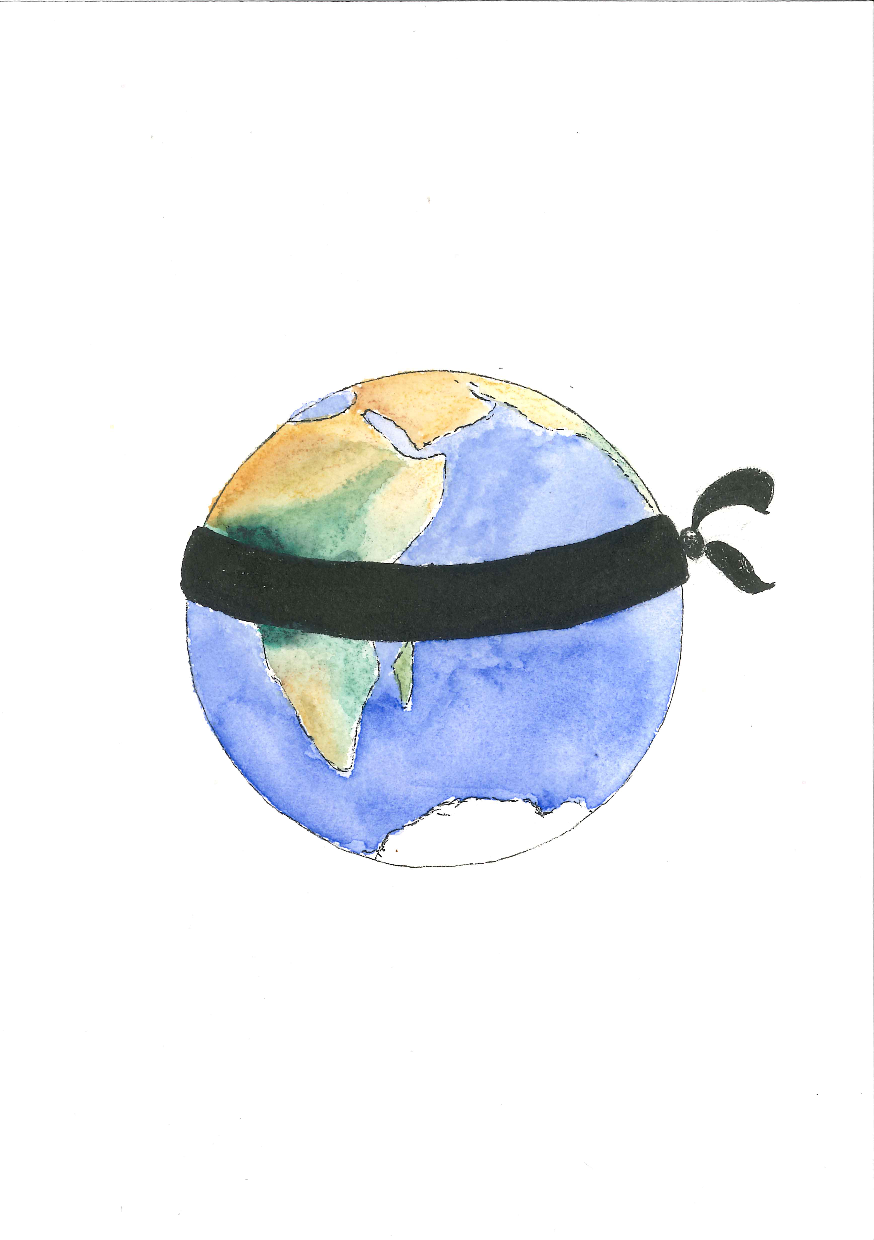
\includegraphics[trim={2mm, 22mm, 2mm, 2mm}, clip, width=0.995\pagewidth]{scans/pan-6.pdf}};
    \begin{scope}[x={(current page.south east)},y={(current page.north west)}]
		\if\helplines1
			\draw[help lines,xstep=.1,ystep=.1] (0,0) grid (\N, \N);
		\else
			\path[help lines,xstep=.1,ystep=.1] (0,0) grid (\N, \N);
		\fi
		\node(title) at (0.5, 0.9) {\Huge {\color{Maroon}V} - \textsc{CASP}};
		
		
		\node[text width=0.4\pagewidth, align=justify, anchor=north west] at (0.075, 0.85) {\english{CASP is a world wide blind test experiment, where research groups submit their predictions to proteins that are still unknown.
		Some months afterwards, the experimental results are published and the community can evaluate how well we performed, in a trully blind test.}};
		
		\node[text width=0.4\pagewidth, align=justify, anchor= west] at (0.075, 0.11) {\english{In this paper we compare the results of ProQ3D and ProQ4 against other people's, and show that our numbers are still consistent.}};
		
		% % % % %
		
		\node[text width=0.4\pagewidth, align=justify, anchor=north east] at (1-0.075, 0.85) {\spanish{\textsc{casp} es un experimento a ciegas a escala mundial, donde divesos grupos de investigación envían sus predicciones acerca de proteínas hasta el momento desconocidas.
		Unos meses después, los resultados experimentales son publicados, y la comunidad puede evaluar qué tal funcionan los métodos. Los resultados son, de esta forma, ciegos y justos.}};
		
		
		\node[text width=0.4\pagewidth, align=justify, anchor=east] at (1-0.075, 0.11) {\spanish{En este artículo comparamos los resultados de ProQ3D y ProQ4 con los de otros grupos, y mostramos que nuestros números son consistentes con nuestros anteriores artículos.}};
    \end{scope}

\end{tikzpicture}
\end{center}
